\begin{figure*}[tp]
\centering
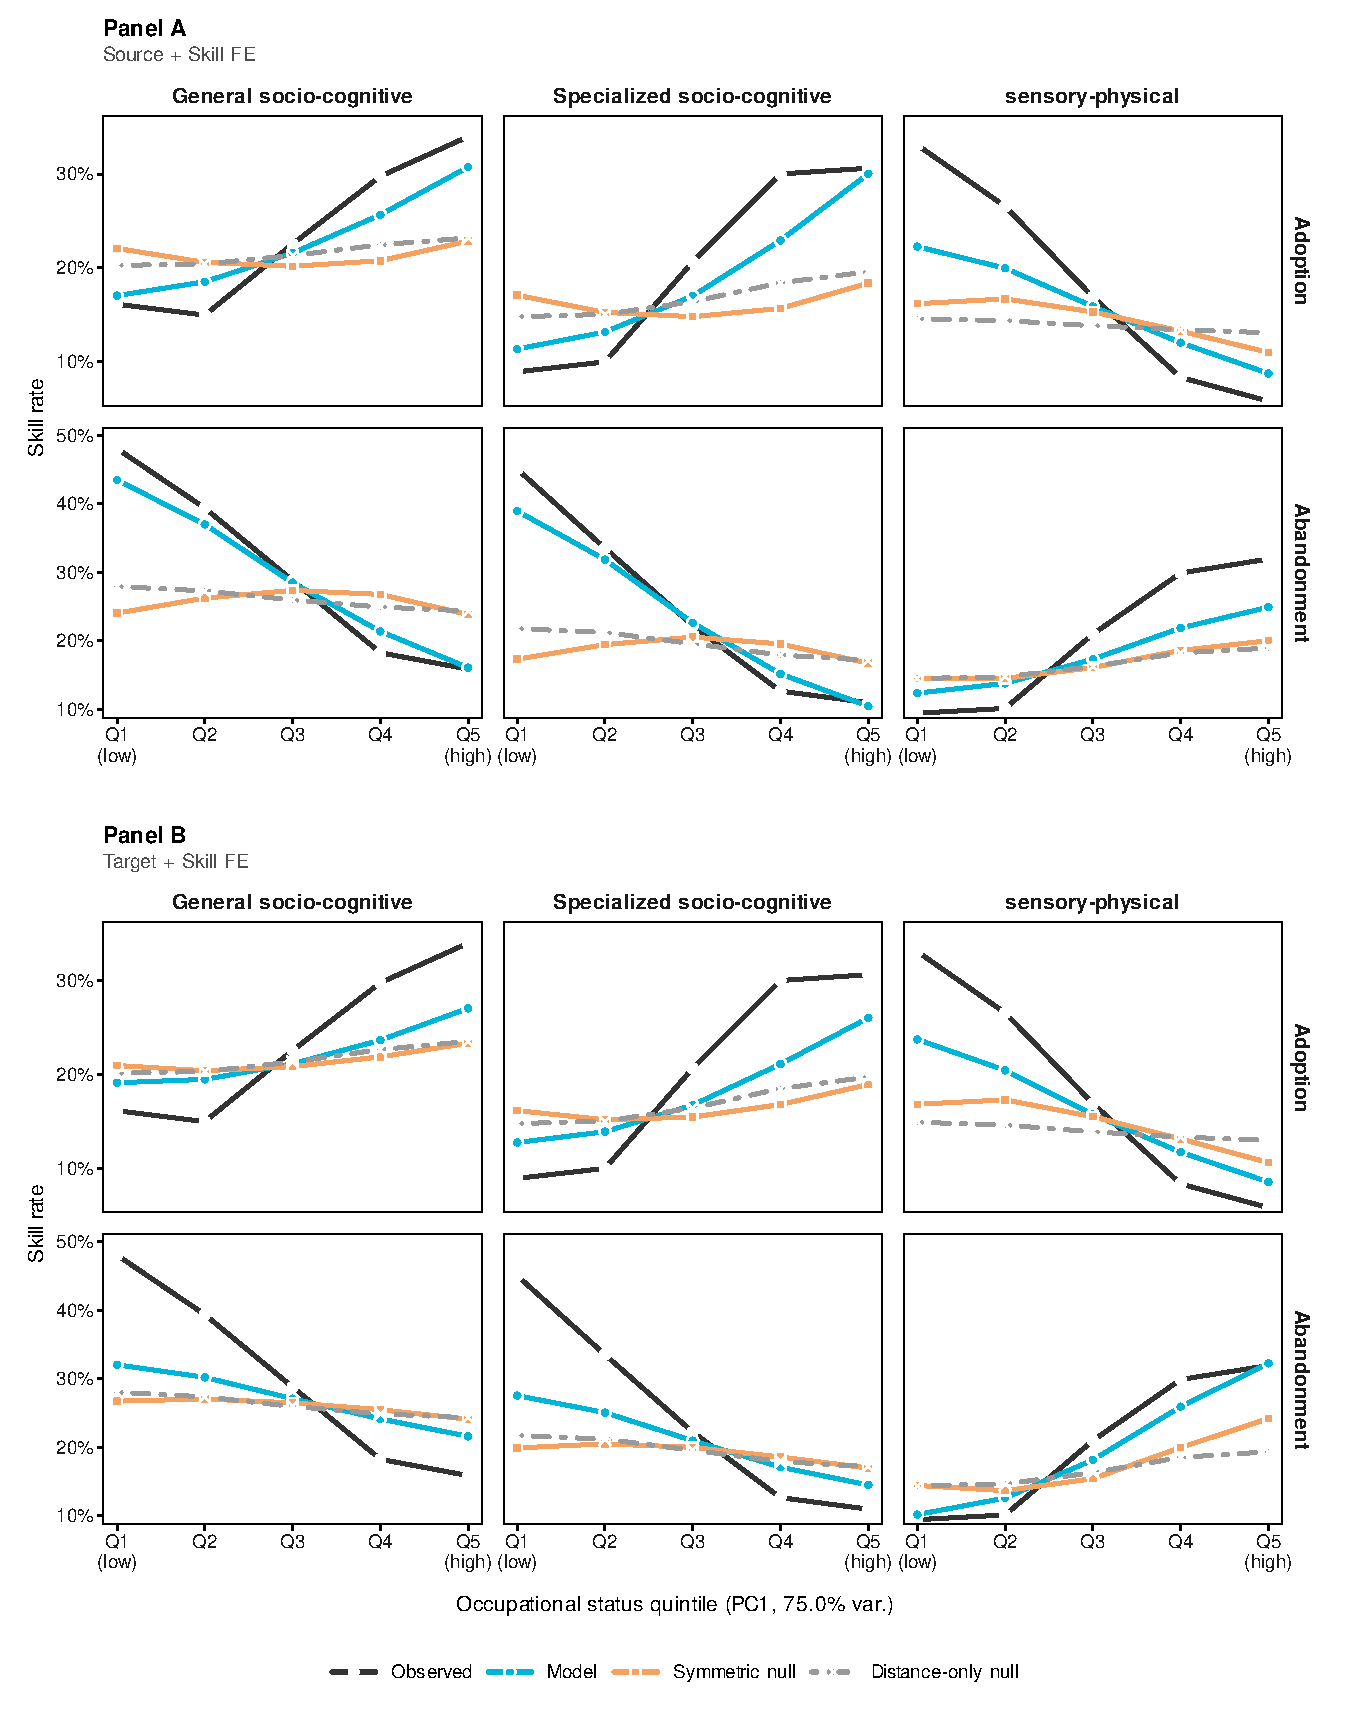
\includegraphics[width=0.85\textwidth]{figures/fig3_unified.pdf}
\caption{%
\textbf{The dyadic directional rule reproduces the aggregate gradient of occupational skill change.}
Observed and model-projected adoption (left) and abandonment (right) rates by occupational status quintile (Q1 = lowest, Q5 = highest) for each skill class, under both complementary fixed-effect strategies: source and skill fixed effects (\textbf{Panel A}, top) and target and skill fixed effects (\textbf{Panel B}, bottom). The directional model applies the full set of estimated channel parameters to every dyad in the risk set and averages within quintiles; the symmetric null retains only the magnitude of the status gap, and the distance-only null only task proximity. Socio-cognitive skills concentrate in higher-status occupations and sensory-physical skills in lower-status ones, and the directional model tracks this gradient under both strategies while the direction-blind nulls stay close to flat. Full Q5--Q1 gradient statistics for both strategies are reported in Table~\ref{tab:SI_gradients} (\hyperref[sec:SI_projections]{Supplementary Section~\ref*{sec:SI_projections}}). O*NET, 2015--2024.
}
\label{fig:projection_main}
\end{figure*}
